\chapter{Highlevel design}
    \section{Operation model}
    JobAdder follows the Client/Server and the Master/Worker architectures:
    \linebreak
    \begin{minipage}[b]{0.5\linewidth}
        \begin{enumerate}
            \item Users operate on their user machines and are Clients.
            \item The central server is both the Server for the User Clients and a Master for the Worker Machines.
            \item Computational nodes are Workers.
        \end{enumerate}
    \end{minipage}
    \hfill
    \begin{minipage}[b]{0.35\linewidth}
        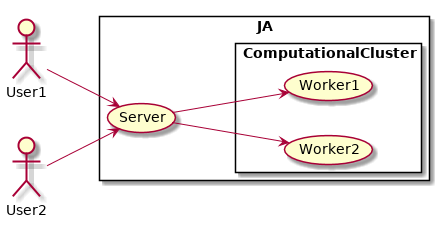
\includegraphics[height=8\baselineskip]{architecture/client-server-worker.png}
    \end{minipage}

    \section{Data flow}
    The data flow inside the Server follows the Pipeline model:
    \linebreak
    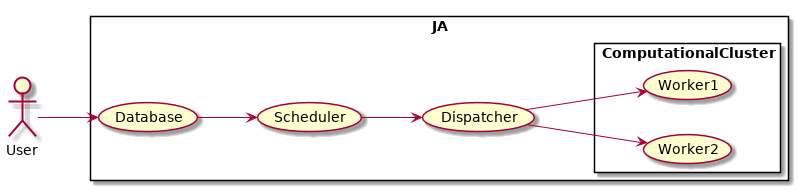
\includegraphics[width=\linewidth]{architecture/server-internal.png}
    \begin{enumerate}
        \item Incoming requests (adding a new job, cancelling a job, etc.) are stored in the Database.
        \item The changes are afterwards processed by the Scheduler.
        \item By using the new job distribution, Dispatcher generates the exact commands to be executed by each Worker.
        \item Commands are sent to the individual workers.
    \end{enumerate}
